% ====================================================================
% ФАЙЛ: tasks/01_mechanics/advanced_mechanics_bank_part1.tex
% ТЕМА: МЕХАНИКА (ВЫСОКИЙ УРОВЕНЬ СЛОЖНОСТИ)
% ПАЧКА 1: ВАРИАНТЫ 1–2
% ====================================================================

% === ЗАДАЧА 1 ===
% Тег: #МЕХАНИКА #КИМ_22 #ВАРИАНТ_01
\begin{taskbasic}[code={\label{task:mechanics_v1_n22}}]
\textbf{Задача 1.} Столкнулись два одинаковых пластилиновых шарика, движущихся по гладкой горизонтальной поверхности, причём векторы их скоростей непосредственно перед столкновением были взаимно перпендикулярны и втрое различались по модулю: $v_1 = 3v_2$. Какова скорость шариков после абсолютно неупругого столкновения, если перед столкновением скорость более быстрого шарика была равна по модулю $6$~м/с?

\kim{22}
\end{taskbasic}
\answer{3,16}

% === ЗАДАЧА 2 ===
% Тег: #МЕХАНИКА #КИМ_26 #ВАРИАНТ_01
\begin{taskbasic}[code={\label{task:mechanics_v1_n26}}]
\textbf{Задача 2.} Тонкий однородный стержень $AB$ постоянного сечения шарнирно закреплён в точке $A$ и удерживается горизонтальной нитью $BC$ (см. рисунок), угол наклона стержня к горизонту $\alpha = 45^{\circ}$. Трение в шарнире пренебрежимо мало. Найдите массу стержня $m$, если модуль силы $F$, с которой шарнир действует на стержень, равен $35$~Н. Сделайте рисунок, на котором укажите все силы, действующие на стержень. Обоснуйте применимость законов, используемых для решения задачи.

\nopagebreak\smallskip
\begin{center}
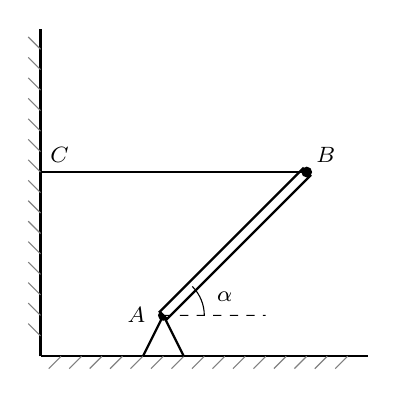
\begin{tikzpicture}[scale=1.3, every node/.style={font=\footnotesize}]
    % Вертикальная стена
    \draw[thick] (0,0) -- (0,3.2);
    \foreach \y in {0.2,0.4,0.6,0.8,1.0,1.2,1.4,1.6,1.8,2.0,2.2,2.4,2.6,2.8,3.0}
        \draw[gray, thin] (0,\y) -- (-0.12,\y+0.12);
        
    % Горизонтальный пол
    \draw[thick] (0,0) -- (3.2,0);
    \foreach \x in {0.2,0.4,0.6,0.8,1.0,1.2,1.4,1.6,1.8,2.0,2.2,2.4,2.6,2.8,3.0}
        \draw[gray, thin] (\x,0) -- (\x-0.12,-0.12);

    % Координаты
    \coordinate (A) at (1.2,0.4);
    \coordinate (B) at (2.6,1.8);
    \coordinate (C) at (0,1.8);

    % Шарнир А
    \draw[thick] (1.0,0) -- (A) -- (1.4,0);
    \fill[black] (A) circle (1.5pt) node[left=3pt] {$A$};

    % Стержень
    \begin{scope}[shift={(A)}, rotate=45]
        \draw[thick, fill=white] (0,-0.05) rectangle (1.98,0.05);
    \end{scope}
    \fill[black] (B) circle (1.5pt) node[above right] {$B$};

    % Нить BC
    \draw[thick] (C) -- (B);
    \node[above right] at (C) {$C$};

    % Угол альфа
    \draw[dashed, thin] (A) -- (2.2,0.4);
    \draw (1.6,0.4) arc (0:45:0.4);
    \node at (1.8,0.58) {$\alpha$};
\end{tikzpicture}
\end{center}

\kim{26}
\end{taskbasic}
\answer{3,13}

% === ЗАДАЧА 3 ===
% Тег: #МЕХАНИКА #КИМ_22 #ВАРИАНТ_02
\begin{taskbasic}[code={\label{task:mechanics_v2_n22}}]
\textbf{Задача 3.} Столкнулись два одинаковых пластилиновых шарика, движущихся по гладкой горизонтальной поверхности, причём векторы их скоростей непосредственно перед столкновением были взаимно перпендикулярны и вдвое различались по модулю: $v_1 = 2v_2$. Какова скорость более медленного шарика перед столкновением, если после абсолютно неупругого столкновения их скорость стала равна по модулю $4{,}5$~м/с?

\kim{22}
\end{taskbasic}
\answer{4}

% === ЗАДАЧА 4 ===
% Тег: #МЕХАНИКА #КИМ_26 #ВАРИАНТ_02
\begin{taskbasic}[code={\label{task:mechanics_v2_n26}}]
\textbf{Задача 2.} Тонкий однородный стержень $AB$ постоянного сечения массой $2{,}7$~кг шарнирно закреплён в точке $A$ и удерживается горизонтальной нитью $BC$ (см. рисунок), угол наклона стержня к горизонту $\alpha = 45^{\circ}$. Трение в шарнире пренебрежимо мало. Найдите модуль силы $F$, с которой шарнир действует на стержень. Сделайте рисунок, на котором укажите все силы, действующие на стержень. Обоснуйте применимость законов, используемых для решения задачи.

\nopagebreak\smallskip
\begin{center}
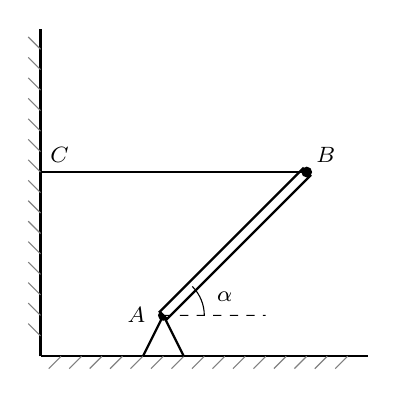
\begin{tikzpicture}[scale=1.3, every node/.style={font=\footnotesize}]
    % Вертикальная стена
    \draw[thick] (0,0) -- (0,3.2);
    \foreach \y in {0.2,0.4,0.6,0.8,1.0,1.2,1.4,1.6,1.8,2.0,2.2,2.4,2.6,2.8,3.0}
        \draw[gray, thin] (0,\y) -- (-0.12,\y+0.12);
        
    % Горизонтальный пол
    \draw[thick] (0,0) -- (3.2,0);
    \foreach \x in {0.2,0.4,0.6,0.8,1.0,1.2,1.4,1.6,1.8,2.0,2.2,2.4,2.6,2.8,3.0}
        \draw[gray, thin] (\x,0) -- (\x-0.12,-0.12);

    % Координаты
    \coordinate (A) at (1.2,0.4);
    \coordinate (B) at (2.6,1.8);
    \coordinate (C) at (0,1.8);

    % Шарнир А
    \draw[thick] (1.0,0) -- (A) -- (1.4,0);
    \fill[black] (A) circle (1.5pt) node[left=3pt] {$A$};

    % Стержень
    \begin{scope}[shift={(A)}, rotate=45]
        \draw[thick, fill=white] (0,-0.05) rectangle (1.98,0.05);
    \end{scope}
    \fill[black] (B) circle (1.5pt) node[above right] {$B$};

    % Нить BC
    \draw[thick] (C) -- (B);
    \node[above right] at (C) {$C$};

    % Угол альфа
    \draw[dashed, thin] (A) -- (2.2,0.4);
    \draw (1.6,0.4) arc (0:45:0.4);
    \node at (1.8,0.58) {$\alpha$};
\end{tikzpicture}
\end{center}

\kim{26}
\end{taskbasic}
\answer{30,2}

% ====================================================================
% ФАЙЛ: tasks/01_mechanics/advanced_mechanics_bank_part2.tex
% ТЕМА: МЕХАНИКА (ВЫСОКИЙ УРОВЕНЬ СЛОЖНОСТИ)
% ПАЧКА 2: ВАРИАНТЫ 3–4
% ====================================================================

% === ЗАДАЧА 1 ===
% Тег: #МЕХАНИКА #КИМ_22 #ВАРИАНТ_03
\begin{taskbasic}[code={\label{task:mechanics_v3_n22}}]
\textbf{Задача 1.} Два пластилиновых шарика массами $m_1 = 15$~г и $m_2 = 25$~г, летящие навстречу друг другу с одинаковыми по модулю скоростями $v_1 = v_2 = 4$~м/с, при столкновении слипаются. Какой становится их скорость сразу после столкновения? Считать, что время взаимодействия шариков мало.

\kim{22}
\end{taskbasic}
\answer{1}

% === ЗАДАЧА 2 ===
% Тег: #МЕХАНИКА #КИМ_26 #ВАРИАНТ_03
\begin{taskbasic}[code={\label{task:mechanics_v3_n26}}]
\textbf{Задача 2.} Однородный рычаг $AB$ может вращаться без трения вокруг неподвижной оси, проходящей через рычаг в точке $O$ перпендикулярно ему. К левому концу рычага в точке $A$ прикреплена нить, за которую с помощью динамометра $D$ рычаг неподвижно удерживается в горизонтальном положении. Нить составляет с вертикалью угол, который можно измерить с помощью транспортира $T$. Показания динамометра (в ньютонах) и транспортира (в градусах) видны на фотографии (угол равен $45^{\circ}$, сила равна $1{,}8$~Н). К точке $C$ с помощью другой невесомой нерастяжимой нити подвешена медная пластина. Рычаг, пластина, нить и динамометр расположены в вертикальной плоскости. Массами транспортира и нитей пренебречь. Определите массу медной пластины, если рычаг имеет массу $30$~г. Сделайте рисунок, на котором укажите все силы, действующие на рычаг и пластину. Обоснуйте применимость законов, используемых для решения задачи.

\nopagebreak\smallskip
\begin{center}
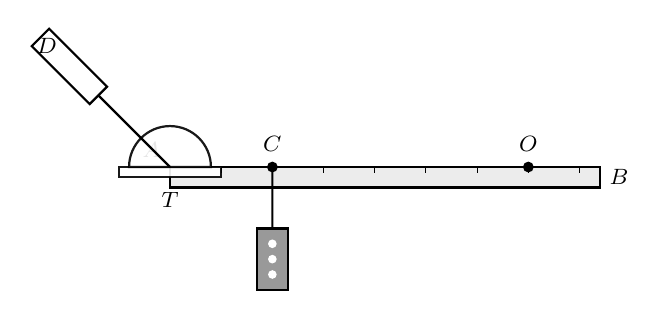
\begin{tikzpicture}[scale=1.3, every node/.style={font=\footnotesize}]
    % Отрезок рычага
    \draw[thick, fill=gray!15] (0,0) rectangle (4.2,-0.2);
    \foreach \x in {0.5,1.0,1.5,2.0,2.5,3.0,3.5,4.0}
        \draw[thin] (\x,0) -- (\x,-0.06);
        
    \coordinate (A) at (0,0);
    \coordinate (C) at (1.0,0);
    \coordinate (O) at (3.5,0);
    
    \fill[black] (O) circle (1.5pt) node[above=2pt] {$O$};
    \fill[black] (C) circle (1.5pt) node[above=2pt] {$C$};
    \node[above left] at (A) {$A$};
    \node[right] at (4.2,-0.1) {$B$};

    % Подвес груза
    \draw[thick] (C) -- (1.0,-0.6);
    \draw[thick, fill=gray!80] (0.85,-0.6) rectangle (1.15,-1.2);
    \foreach \y in {-0.75,-0.9,-1.05} \fill[white] (1.0,\y) circle (1.2pt);

    % Транспортир
    \begin{scope}[shift={(A)}]
        \draw[thick, fill=white, opacity=0.9] (-0.5,-0.1) rectangle (0.5,0);
        \draw[thick, fill=white, opacity=0.9] (0.4,0) arc (0:180:0.4) -- cycle;
        \node[below=2pt] at (0,-0.1) {$T$};
    \end{scope}

    % Нить под углом 45 к вертикали (135 градусов)
    \draw[thick] (A) -- (-0.7,0.7);
    \begin{scope}[shift={(-0.7,0.7)}, rotate=45]
        \draw[thick, fill=white] (-0.12,0) rectangle (0.12,0.8);
        \node[above left=1pt] at (0,0.4) {$D$};
    \end{scope}
\end{tikzpicture}
\end{center}

\kim{26}
\end{taskbasic}
\answer{0{,}35}

% === ЗАДАЧА 3 ===
% Тег: #МЕХАНИКА #КИМ_22 #ВАРИАНТ_04
\begin{taskbasic}[code={\label{task:mechanics_v4_n22}}]
\textbf{Задача 3.} Два пластилиновых шарика массами $m_1 = 20$~г и $m_2 = 30$~г, летящие навстречу друг другу со скоростями $v_1 = 4$~м/с и $v_2 = 3$~м/с, при столкновении слипаются. Какой становится их скорость сразу после столкновения? Считать, что время взаимодействия шариков мало.

\kim{22}
\end{taskbasic}
\answer{0{,}2}

% === ЗАДАЧА 4 ===
% Тег: #МЕХАНИКА #КИМ_26 #ВАРИАНТ_04
\begin{taskbasic}[code={\label{task:mechanics_v4_n26}}]
\textbf{Задача 4.} Однородный рычаг $AB$ может вращаться без трения вокруг неподвижной оси, проходящей через рычаг в точке $O$ перпендикулярно ему. К левому концу рычага в точке $A$ прикреплена нить, за которую с помощью динамометра $D$ рычаг неподвижно удерживается в горизонтальном положении. Нить составляет с вертикалью угол, который можно измерить с помощью транспортира $T$. Показания динамометра (в ньютонах) и транспортира (в градусах) видны на фотографии (угол равен $45^{\circ}$, сила равна $1{,}8$~Н). К точке $C$ с помощью другой невесомой нерастяжимой нити подвешена латунная пластина. Рычаг, пластина, нить и динамометр расположены в вертикальной плоскости. Массами транспортира и нитей пренебречь. Определите массу рычага, если латунная пластина имеет массу $120$~г. Сделайте рисунок, на котором укажите все силы, действующие на рычаг и пластину. Обоснуйте применимость законов, используемых для решения задачи.

\nopagebreak\smallskip
\begin{center}
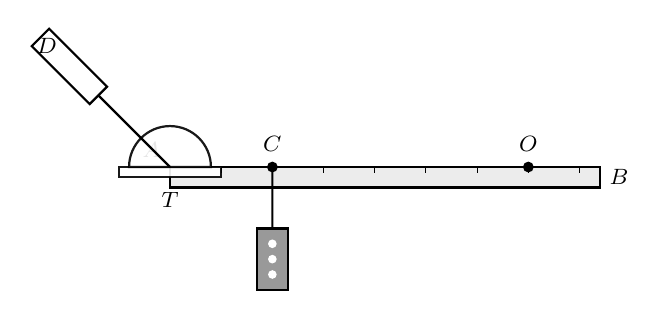
\begin{tikzpicture}[scale=1.3, every node/.style={font=\footnotesize}]
    % Отрезок рычага
    \draw[thick, fill=gray!15] (0,0) rectangle (4.2,-0.2);
    \foreach \x in {0.5,1.0,1.5,2.0,2.5,3.0,3.5,4.0}
        \draw[thin] (\x,0) -- (\x,-0.06);
        
    \coordinate (A) at (0,0);
    \coordinate (C) at (1.0,0);
    \coordinate (O) at (3.5,0);
    
    \fill[black] (O) circle (1.5pt) node[above=2pt] {$O$};
    \fill[black] (C) circle (1.5pt) node[above=2pt] {$C$};
    \node[above left] at (A) {$A$};
    \node[right] at (4.2,-0.1) {$B$};

    % Подвес груза
    \draw[thick] (C) -- (1.0,-0.6);
    \draw[thick, fill=gray!80] (0.85,-0.6) rectangle (1.15,-1.2);
    \foreach \y in {-0.75,-0.9,-1.05} \fill[white] (1.0,\y) circle (1.2pt);

    % Транспортир
    \begin{scope}[shift={(A)}]
        \draw[thick, fill=white, opacity=0.9] (-0.5,-0.1) rectangle (0.5,0);
        \draw[thick, fill=white, opacity=0.9] (0.4,0) arc (0:180:0.4) -- cycle;
        \node[below=2pt] at (0,-0.1) {$T$};
    \end{scope}

    % Нить под углом 45 к вертикали (135 градусов)
    \draw[thick] (A) -- (-0.7,0.7);
    \begin{scope}[shift={(-0.7,0.7)}, rotate=45]
        \draw[thick, fill=white] (-0.12,0) rectangle (0.12,0.8);
        \node[above left=1pt] at (0,0.4) {$D$};
    \end{scope}
\end{tikzpicture}
\end{center}

\kim{26}
\end{taskbasic}
\answer{0{,}06}

% ====================================================================
% ФАЙЛ: tasks/01_mechanics/advanced_mechanics_bank_part3.tex
% ТЕМА: МЕХАНИКА (ВЫСОКИЙ УРОВЕНЬ СЛОЖНОСТИ)
% ПАЧКА 3: ВАРИАНТЫ 5–6
% ====================================================================

% === ЗАДАЧА 1 ===
% Тег: #МЕХАНИКА #КИМ_22 #ВАРИАНТ_05
\begin{taskbasic}[code={\label{task:mechanics_v5_n22}}]
\textbf{Задача 1.} Тележка массой $40$~кг движется со скоростью, равной по модулю $1$~м/с, слева направо по гладкой горизонтальной дороге. Каким станет модуль скорости тележки, если человек массой $60$~кг запрыгнет на тележку со скоростью, равной по модулю $2$~м/с относительно дороги и направленной слева направо?

\kim{22}
\end{taskbasic}
\answer{1{,}6}

% === ЗАДАЧА 2 ===
% Тег: #МЕХАНИКА #КИМ_26 #ВАРИАНТ_05
\begin{taskbasic}[code={\label{task:mechanics_v5_n26}}]
\textbf{Задача 2.} Два сплошных груза массами $1{,}28$~кг и $0{,}32$~кг подвесили за невесомые нерастяжимые нити к концам невесомого рычага и привели рычаг в состояние равновесия. Затем рычаг с грузами расположили над керосином так, что оба груза целиком оказались в керосине. В результате для сохранения равновесия точку опоры пришлось переместить на $10$~см. Определите первоначальное расстояние от более тяжёлого груза до точки опоры, если объёмы обоих грузов одинаковы и равны $250\text{ см}^3$. Плотность керосина примите равной $800\text{ кг/м}^3$. Сделайте рисунок, на котором укажите силы, действующие на рычаг для двух случаев, а также на погружённые в керосин грузы. Обоснуйте применимость законов, используемых для решения задачи.

\kim{26}
\end{taskbasic}
\answer{0{,}16}

% === ЗАДАЧА 3 ===
% Тег: #МЕХАНИКА #КИМ_22 #ВАРИАНТ_06
\begin{taskbasic}[code={\label{task:mechanics_v6_n22}}]
\textbf{Задача 3.} Тележка массой $60$~кг движется со скоростью, равной по модулю $1$~м/с, слева направо по гладкой горизонтальной дороге. Каким станет модуль скорости тележки, если девочка массой $40$~кг запрыгнет на тележку со скоростью, равной по модулю $2$~м/с относительно дороги и направленной слева направо?

\kim{22}
\end{taskbasic}
\answer{1{,}4}

% === ЗАДАЧА 4 ===
% Тег: #МЕХАНИКА #КИМ_26 #ВАРИАНТ_06
\begin{taskbasic}[code={\label{task:mechanics_v6_n26}}]
\textbf{Задача 4.} К концам невесомого рычага подвесили за невесомые нерастяжимые нити два сплошных груза массами $1{,}28$~кг и $0{,}32$~кг и привели рычаг в состояние равновесия. Затем рычаг с грузами расположили над водой так, что оба груза целиком оказались под водой. Первоначальное расстояние от более тяжёлого груза до точки опоры равно $20$~см. Определите, на сколько необходимо переместить точку опоры для сохранения равновесия, если объёмы обоих грузов одинаковы и равны $200\text{ см}^3$. Плотность воды примите равной $1000\text{ кг/м}^3$. Сделайте рисунок, на котором укажите силы, действующие на рычаг для двух случаев, а также на погружённые в воду грузы. Обоснуйте применимость законов, используемых для решения задачи.

\kim{26}
\end{taskbasic}
\answer{0{,}04}

% ====================================================================
% ФАЙЛ: tasks/01_mechanics/advanced_mechanics_bank_part4.tex
% ТЕМА: МЕХАНИКА (ВЫСОКИЙ УРОВЕНЬ СЛОЖНОСТИ)
% ПАЧКА 4: ВАРИАНТЫ 7–8
% ====================================================================

% === ЗАДАЧА 1 ===
% Тег: #МЕХАНИКА #КИМ_26 #ВАРИАНТ_07
\begin{taskbasic}[code={\label{task:mechanics_v7_n26}}]
\textbf{Задача 1.} Небольшое тело массой $M = 0{,}99$~кг лежит на вершине гладкой полусферы радиусом $R$. В тело попадает пуля массой $m = 0{,}01$~кг, летящая горизонтально со скоростью $v_0 = 200$~м/с, и застревает в нём. Пренебрегая смещением тела за время удара, определите радиус полусферы $R$, если известно, что высота, на которой это тело оторвётся от поверхности полусферы, составила $h = 1$~м. Высота отсчитывается от основания полусферы. Сопротивлением воздуха пренебречь. Обоснуйте применимость законов, используемых для решения задачи.

\kim{26}
\end{taskbasic}
\answer{1{,}3}

% === ЗАДАЧА 2 ===
% Тег: #МЕХАНИКА #КИМ_26 #ВАРИАНТ_08
\begin{taskbasic}[code={\label{task:mechanics_v8_n26}}]
\textbf{Задача 2.} Небольшое тело массой $M = 0{,}99$~кг лежит на вершине гладкой полусферы радиусом $R = 1$~м. В тело попадает пуля массой $m = 0{,}01$~кг, летящая горизонтально со скоростью $v_0 = 200$~м/с, и застревает в нём. Пренебрегая смещением тела за время удара, определите высоту $h$, на которой это тело оторвётся от поверхности полусферы. Высота отсчитывается от основания полусферы. Сопротивлением воздуха пренебречь. Обоснуйте применимость законов, используемых для решения задачи.

\kim{26}
\end{taskbasic}
\answer{0{,}8}

% ====================================================================
% ФАЙЛ: tasks/01_mechanics/advanced_mechanics_bank_part5.tex
% ТЕМА: МЕХАНИКА (ВЫСОКИЙ УРОВЕНЬ СЛОЖНОСТИ)
% ПАЧКА 5: ВАРИАНТЫ 9–10 (АКТУАЛИЗИРОВАННАЯ)
% ====================================================================

% === ЗАДАЧА 1 ===
% Тег: #МЕХАНИКА #КИМ_22 #ВАРИАНТ_09
\begin{taskbasic}[code={\label{task:mechanics_v9_n22_fixed}}]
\textbf{Задача 1.} При упругой деформации, равной $2$~см, потенциальная энергия пружины равна $10$~мДж. На сколько увеличится потенциальная энергия этой пружины при увеличении упругой деформации ещё на $2$~см?

\kim{22}
\end{taskbasic}
\answer{30}

% === ЗАДАЧА 2 ===
% Тег: #МЕХАНИКА #КИМ_26 #ВАРИАНТ_09
\begin{taskadvanced}[code={\label{task:mechanics_v9_n26_fixed}}]
\textbf{Задача 2.} 
Однородный брусок $AB$ массой $M$ постоянного прямоугольного сечения лежит на гладкой горизонтальной поверхности стола, свешиваясь с него менее чем наполовину (см. рисунок). К правому концу бруска прикреплена невесомая нерастяжимая нить. Другой конец нити закреплён на меньшем из двух дисков невесомого составного блока. На большем диске этого блока закреплена другая невесомая нерастяжимая нить, на которой висит груз массой $m$. Диски скреплены друг с другом и образуют единое целое, $R = 12\text{ см}$, $r = 8\text{ см}$. Найдите минимальное значение отношения $\frac{M}{m}$, при котором система тел остаётся неподвижной. Трением в оси блока пренебречь. Сделайте рисунок, на котором укажите все силы, действующие на брусок, груз и блок. Обоснуйте применимость законов, используемых для решения задачи.

\nopagebreak\smallskip
\begin{center}
\begin{tikzpicture}[>=Stealth, scale=1.2]
    % --- Поверхность стола со штриховкой ---
    \fill[pattern=north west lines, pattern color=brandSecondary!30] (0,-0.2) rectangle (4,0);
    \fill[pattern=north west lines, pattern color=brandSecondary!30] (3.8,-1.2) rectangle (4,0);
    \draw[thick, color=brandSecondary] (0,0) -- (4,0) -- (4,-1.2);

    % --- Брусок AB ---
    \draw[thick, fill=white, color=brandSecondary] (0.6,0) rectangle (4.6,0.2);
    \node[above left, inner sep=1pt, font=\footnotesize] at (0.6,0.2) {$A$};
    \node[above right, inner sep=1pt, font=\footnotesize] at (4.6,0.2) {$B$};
    \node[above, font=\footnotesize] at (2.6,0.2) {$M$};

    % --- Составной блок ---
    \coordinate (O) at (5.2, 2.2);
    % Большой диск R
    \draw[thick, color=brandSecondary] (O) circle (1.2);
    % Меньший диск r (левый край касается линии x = 4.6)
    \draw[thick, color=brandSecondary] (O) circle (0.6);
    \fill[color=brandSecondary] (O) circle (1.5pt);

    % Подвес блока к потолку
    \fill[pattern=north west lines, pattern color=brandSecondary!30] (4.8,3.5) rectangle (5.6,3.7);
    \draw[thick, color=brandSecondary] (4.8,3.5) -- (5.6,3.5);
    \draw[thick, color=brandSecondary] (4.9,2.2) -- (4.9,3.5) -- (5.5,3.5) -- (5.5,2.2);

    % --- Нити ---
    % Левая нить (от бруска к малому диску)
    \draw[thick, color=brandSecondary] (4.6,0.2) -- (4.6,2.2);
    % Правая нить (от большого диска к грузу m)
    \draw[thick, color=brandSecondary] (6.4,2.2) -- (6.4,0.8);

    % --- Груз m ---
    \draw[thick, fill=white, color=brandSecondary] (6.1,0.2) rectangle (6.7,0.8);
    \node[right] at (6.7,0.5) {$m$};

    % --- Указатели радиусов (как на исходном рисунке) ---
    \draw[thin, <-] (4.95,2.5) -- (4.2,2.8) node[left, font=\footnotesize] {$r$};
    \draw[thin, <-] (4.4,1.4) -- (3.9,1.1) node[left, font=\footnotesize] {$R$};

    % --- ВЕКТОРЫ СИЛ (выделены brandPrimary) ---
    % На груз m
    \draw[->, very thick, color=brandPrimary] (6.4,0.5) -- (6.4,1.1) node[right] {$\vec{T}_2$};
    \draw[->, very thick, color=brandPrimary] (6.4,0.5) -- (6.4,-0.2) node[right] {$m\vec{g}$};

    % На блок
    \draw[->, very thick, color=brandPrimary] (4.6,2.2) -- (4.6,1.6) node[left] {$\vec{T}'_1$};
    \draw[->, very thick, color=brandPrimary] (6.4,2.2) -- (6.4,1.6) node[right] {$\vec{T}'_2$};
    \draw[->, very thick, color=brandPrimary] (O) -- (5.2, 2.9) node[right] {$\vec{F}_{\text{оси}}$};

    % На брусок
    \draw[->, very thick, color=brandPrimary] (4.6,0.2) -- (4.6,0.9) node[left] {$\vec{T}_1$};
    \draw[->, very thick, color=brandPrimary] (2.6,0.1) -- (2.6,-0.5) node[right] {$M\vec{g}$};
    \draw[->, very thick, color=brandPrimary] (2.0,0.0) -- (2.0,0.6) node[left] {$\vec{N}$};

\end{tikzpicture}
\end{center}

\begin{solutionbox}
\textbf{Обоснование применимости законов:}
\begin{enumerate}[leftmargin=*]
    \item Рассмотрим систему тел в инвариантной ИСО, связанной с Землёй.
    \item Брусок и подвешенный груз моделируем как твердые тела. Условием их неподвижности (равновесия) является равенство нулю геометрической суммы всех внешних сил, а для бруска — также и равенство нулю суммы моментов сил относительно любой оси.
    \item Так как нити являются невесомыми и нерастяжимыми, а трение в оси блока отсутствует, модуль силы натяжения вдоль каждой из нитей постоянен: $T_1 = T'_1$ и $T_2 = T'_2$.
\end{enumerate}

\textbf{Решение:}
1. Рассмотрим условие равновесия груза массой $m$ в проекции на вертикальную ось:
$$T_2 - mg = 0 \implies T_2 = mg$$

2. Блок является невесомым, поэтому сумма моментов сил, действующих на него относительно оси вращения, проходящей через центр $O$, равна нулю:
$$T'_2 \cdot R - T'_1 \cdot r = 0$$
Учитывая, что $T'_2 = T_2 = mg$ и $T'_1 = T_1$, получаем выражение для силы натяжения левой нити:
$$mg \cdot R - T_1 \cdot r = 0 \implies T_1 = mg \frac{R}{r}$$

3. Рассмотрим силы, действующие на брусок массой $M$. На него действуют: сила тяжести $M\vec{g}$ (приложена к центру бруска), сила натяжения нити $\vec{T}_1$ (приложена к правому краю $B$) и сила нормальной реакции стола $\vec{N}$ (направлена вертикально вверх).

Запишем условие баланса сил для бруска в проекции на вертикальную ось:
$$N + T_1 - Mg = 0 \implies N = Mg - T_1$$

4. Поскольку поверхность стола не может «притягивать» брусок (она удерживает его только за счёт силы реакции, направленной вверх), сила нормального давления должна строго удовлетворять условию неотрицательности:
$$N \ge 0 \implies Mg - T_1 \ge 0 \implies T_1 \le Mg$$

Если это условие нарушится ($T_1 > Mg$), направленная вверх сила натяжения нити на правом конце превысит полную силу тяжести бруска, и он неминуемо оторвётся от стола, начав движение вверх, независимо от величины его свеса.

5. Подставим ранее найденное значение силы $T_1$ в полученное неравенство:
$$mg \frac{R}{r} \le Mg \implies \frac{M}{m} \ge \frac{R}{r}$$

6. Таким образом, минимально возможное отношение масс, гарантирующее неподвижность системы при любых начальных условиях расположения центра масс на гладком столе, составляет:
$$\left(\frac{M}{m}\right)_{\text{min}} = \frac{R}{r} = \frac{12}{8} = 1{,}5$$
\end{solutionbox}


\kim{26}
\end{taskadvanced}
\answer{1,5}
% === ЗАДАЧА 3 ===
% Тег: #МЕХАНИКА #КИМ_22 #ВАРИАНТ_10
\begin{taskbasic}[code={\label{task:mechanics_v10_n22_fixed}}]
\textbf{Задача 3.} При прямолинейном движении по горизонтальной поверхности на брусок массой $40$~кг действует сила трения скольжения, равная по модулю $80$~Н. Во сколько раз необходимо увеличить массу бруска, чтобы при неизменном коэффициенте трения модуль силы трения скольжения был равен $120$~Н?

\kim{22}
\end{taskbasic}
\answer{1{,}5}

% === ЗАДАЧА 4 ===
% Тег: #МЕХАНИКА #КИМ_26 #ВАРИАНТ_10
\begin{taskbasic}[code={\label{task:mechanics_v10_n26_fixed}}]
\textbf{Задача 4.} Однородный рычаг $AB$ может вращаться без трения вокруг неподвижной оси, проходящей через рычаг в точке $O$ перпендикулярно ему. К левому концу рычага в точке $A$ прикреплена нить, за которую с помощью динамометра $D$ рычаг неподвижно удерживается в горизонтальном положении. Нить составляет с вертикалью угол, который можно измерить с помощью транспортира $T$. Показания динамометра (в ньютонах) и транспортира (в градусах) видны на фотографии. К точке $C$ с помощью другой невесомой нерастяжимой нити подвешена латунная пластина (см. фотографию). Рычаг, пластина, нить и динамометр расположены в вертикальной плоскости. Массами транспортира и нитей пренебречь. Определите массу рычага, если латунная пластина имеет массу $120$~г. Сделайте рисунок, на котором укажите все силы, действующие на рычаг и пластину. Обоснуйте применимость законов, используемых для решения задачи.

\nopagebreak\smallskip
\begin{center}
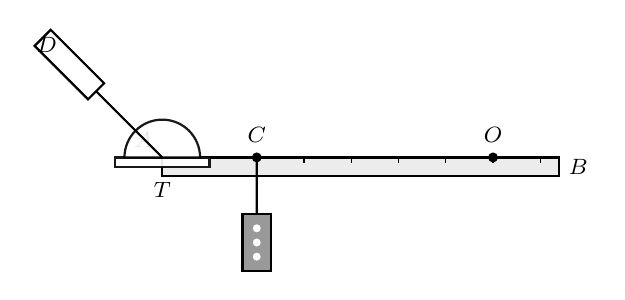
\begin{tikzpicture}[scale=1.2, every node/.style={font=\footnotesize}]
    % Отрезок рычага
    \draw[thick, fill=gray!15] (0,0) rectangle (4.2,-0.2);
    \foreach \x in {0.5,1.0,1.5,2.0,2.5,3.0,3.5,4.0}
        \draw[thin] (\x,0) -- (\x,-0.06);
        
    \coordinate (A) at (0,0);
    \coordinate (C) at (1.0,0);
    \coordinate (O) at (3.5,0);
    
    \fill[black] (O) circle (1.5pt) node[above=2pt] {$O$};
    \fill[black] (C) circle (1.5pt) node[above=2pt] {$C$};
    \node[above left] at (A) {$A$};
    \node[right] at (4.2,-0.1) {$B$};

    % Подвес груза
    \draw[thick] (C) -- (1.0,-0.6);
    \draw[thick, fill=gray!80] (0.85,-0.6) rectangle (1.15,-1.2);
    \foreach \y in {-0.75,-0.9,-1.05} \fill[white] (1.0,\y) circle (1.2pt);

    % Транспортир
    \begin{scope}[shift={(A)}]
        \draw[thick, fill=white, opacity=0.9] (-0.5,-0.1) rectangle (0.5,0);
        \draw[thick, fill=white, opacity=0.9] (0.4,0) arc (0:180:0.4) -- cycle;
        \node[below=2pt] at (0,-0.1) {$T$};
    \end{scope}

    % Нить под углом 45 к вертикали (135 градусов)
    \draw[thick] (A) -- (-0.7,0.7);
    \begin{scope}[shift={(-0.7,0.7)}, rotate=45]
        \draw[thick, fill=white] (-0.12,0) rectangle (0.12,0.8);
        \node[above left=1pt] at (0,0.4) {$D$};
    \end{scope}
\end{tikzpicture}
\end{center}

\kim{26}
\end{taskbasic}
\answer{3}

% ====================================================================
% ФАЙЛ: tasks/01_mechanics/advanced_mechanics_bank_part6.tex
% ТЕМА: МЕХАНИКА (ВЫСОКИЙ УРОВЕНЬ СЛОЖНОСТИ)
% ПАЧКА 6: ВАРИАНТЫ 11–12
% ====================================================================

% === ЗАДАЧА 1 ===
% Тег: #МЕХАНИКА #КИМ_22 #ВАРИАНТ_11
\begin{taskbasic}[code={\label{task:mechanics_v11_n22}}]
\textbf{Задача 1.} Автомобиль массой $1000$~кг движется по горизонтальной дороге. Под действием постоянной тормозящей силы за время $t = 4$~с кинетическая энергия автомобиля уменьшилась в $4$ раза. Определите модуль тормозящей силы, если начальный импульс автомобиля составлял $16000\text{ кг}\cdot\text{м/с}$.

\kim{22}
\end{taskbasic}
\answer{2000}

\begin{taskmedium}
Маленький шарик, подвешенный к потолку на лёгкой нерастяжимой нити, совершает колебания в вертикальной плоскости. Максимальное отклонение нити от вертикали составляет угол $\alpha = 45^\circ$. Сделайте рисунок с указанием сил, приложенных к шарику в тот момент, когда шарик движется вправо-вниз, а нить образует угол $\beta = 30^\circ$ с вертикалью (см. рисунок). Покажите на рисунке, куда направлено в этот момент ускорение шарика (по нити, перпендикулярно нити, внутрь траектории, наружу от траектории). Ответ обоснуйте. Сопротивление воздуха не учитывать.

\nopagebreak\smallskip
\begin{center}
\begin{tikzpicture}[>=Stealth, scale=1.3, font=\small]
    % Потолок со штриховкой
    \fill[pattern=north west lines, pattern color=brandSecondary!30] (-2, 3) rectangle (2, 3.2);
    \draw[thick, color=brandSecondary] (-2, 3) -- (2, 3);
    
    % Точка подвеса О
    \coordinate (O) at (0,3);
    \fill[color=brandSecondary] (O) circle (1.5pt);
    
    % Вспомогательная вертикальная ось (ось симметрии)
    \draw[dashed, color=brandSecondary!60] (0,3) -- (0,0);
    
    % Траектория движения (дуга окружности радиуса R = 2.5)
    \draw[dashed, color=brandSecondary!60] (-45:2.5) [shift={(O)}] arc (-135:-45:2.5);

    % Крайние положения (пунктирные шарики)
    \coordinate (LeftExtreme) at ($(O) + (-135:2.5)$);
    \coordinate (RightExtreme) at ($(O) + (-45:2.5)$);
    \draw[dashed, color=brandSecondary!60] (O) -- (LeftExtreme);
    \draw[dashed, color=brandSecondary!60] (O) -- (RightExtreme);
    \draw[dashed, color=brandSecondary!60, fill=white] (LeftExtreme) circle (0.15);
    \draw[dashed, color=brandSecondary!60, fill=white] (RightExtreme) circle (0.15);

    % Текущее положение: угол beta = 30 градусов от вертикали влево (направление -120 градусов)
    \coordinate (Ball) at ($(O) + (-120:2.5)$);
    
    % Нить к текущему положению
    \draw[thick, color=brandSecondary] (O) -- (Ball);
    
    % Углы alpha и beta
    \draw[thin, color=brandSecondary] (0, 2.0) arc (-90:-135:1.0);
    \node[color=brandSecondary, left] at (-112:1.1) {$\alpha$};
    
    \draw[thin, color=brandSecondary] (0, 2.3) arc (-90:-120:0.7);
    \node[color=brandSecondary, left, yshift=-3pt] at (-105:0.75) {$\beta$};

    % --- ВЕКТОРЫ СИЛ И УСКОРЕНИЯ (brandPrimary) ---
    % Сила тяжести mg (вертикально вниз)
    \draw[->, very thick, color=brandPrimary] (Ball) -- ($(Ball) + (0, -1.2)$) 
        node[below] {$m\vec{g}$};
        
    % Сила натяжения нити T (вдоль нити к точке O)
    % Направление от Ball к O: (0.5, 0.866)
    \draw[->, very thick, color=brandPrimary] (Ball) -- ($(Ball) + (0.65, 1.13)$) 
        node[right, xshift=2pt] {$\vec{T}$};

    % Вектор скорости v (по касательной вправо-вниз: под углом -30 градусов к горизонту)
    % Направление: (0.866, -0.5)
    \draw[->, thick, color=brandSecondary] (Ball) -- ($(Ball) + (0.95, -0.55)$) 
        node[right] {$\vec{v}$};

    % Полное ускорение а (направлено внутрь траектории)
    \draw[->, very thick, color=brandPrimary] (Ball) -- ($(Ball) + (0.85, 0.2)$) 
        node[above right] {$\vec{a}$};

    % Шарик (рисуем поверх векторов для аккуратности)
    \draw[thick, fill=brandSecondary!40, color=brandSecondary] (Ball) circle (0.15);

\end{tikzpicture}
\end{center}

\begin{solutionbox}
\textbf{Обоснование и ход решения:}

1. На шарик действуют две силы: сила тяжести $m\vec{g}$, направленная вертикально вниз, и сила натяжения нити $\vec{T}$, направленная вдоль нити к точке подвеса.

2. Движение шарика происходит по дуге окружности, то есть является криволинейным и неравномерным. Полное ускорение шарика $\vec{a}$ складывается из двух составляющих: центростремительного (нормального) $\vec{a}_n$ и тангенциального (касательного) $\vec{a}_\tau$ ускорений:
$$\vec{a} = \vec{a}_n + \vec{a}_\tau$$

3. **Центростремительное ускорение** определяется мгновенной скоростью движения: $a_n = \frac{v^2}{R}$. Поскольку шарик уже прошёл крайнее левое положение, под действием возвращающей силы он успел разогнаться, его скорость $v \neq 0$. Следовательно, $a_n > 0$, и этот вектор направлен вдоль нити к точке подвеса (в центр окружности).

4. **Тангенциальное ускорение** отвечает за изменение модуля скорости и вызывается проекцией силы тяжести на касательную к траектории: $a_\tau = g \sin\beta$. Так как шарик движется из крайнего положения вниз (к положению равновесия), его скорость увеличивается. Это означает, что вектор $\vec{a}_\tau$ сонаправлен с вектором скорости $\vec{v}$ (направлен по касательной вправо-вниз).

5. Полное ускорение $\vec{a}$ является геометрической суммой взаимно перпендикулярных векторов $\vec{a}_n$ (вдоль нити вверх) и $\vec{a}_\tau$ (по касательной вправо-вниз). В результате сложения этих векторов результирующий вектор ускорения $\vec{a}$ будет направлен **внутрь траектории** (в область между нитью и касательной).
\end{solutionbox}


\kim{21}
\end{taskmedium}
\answer{внутрь траектории}

\begin{taskadvanced}
Однородный тонкий стержень массой $m$ одним концом шарнирно прикреплён к потолку, а другим концом опирается на массивную горизонтальную доску, образуя с ней угол $\alpha = 30^\circ$. Под действием горизонтальной силы $\vec{F}$ доска движется поступательно влево с постоянной скоростью (см. рисунок). Стержень при этом неподвижен. Найдите $m$, если $F = 2\text{ Н}$, а коэффициент трения стержня по доске $\mu = 0{,}2$. Сделайте рисунок с указанием сил, действующих на стержень и доску. Трением доски по опоре и трением в шарнире пренебречь. Обоснуйте применимость законов, используемых для решения задачи.

\nopagebreak\smallskip
\begin{center}
\begin{tikzpicture}[>=Stealth, scale=1.2, font=\small]
    % --- Потолок и опора стола со штриховкой ---
    \fill[pattern=north west lines, pattern color=brandSecondary!30] (2,3) rectangle (5,3.2);
    \draw[thick, color=brandSecondary] (2,3) -- (5,3);
    
    \fill[pattern=north west lines, pattern color=brandSecondary!30] (-1,-0.2) rectangle (5,0);
    \draw[thick, color=brandSecondary] (-1,0) -- (5,0);

    % --- Шарнир на потолке ---
    \coordinate (O) at (4.5,3);
    \draw[thick, color=brandSecondary] (4.5,3) -- (4.3,2.6) -- (4.7,2.6) -- cycle;
    \fill[color=brandSecondary] (O) circle (1.5pt);

    % --- Доска ---
    \draw[thick, fill=white, color=brandSecondary] (-0.5,0) rectangle (4.0,0.6);
    \draw[->, thick, color=brandSecondary] (3.5,0.9) -- (2.3,0.9) node[above, midway] {$\vec{v} = \text{const}$};

    % --- Стержень ---
    % Точные тригонометрические координаты для угла 30 градусов
    \coordinate (A) at (1.04, 0.6);
    \coordinate (B) at (4.5, 2.6);
    \draw[ultra thick, color=brandSecondary] (A) -- (B);
    \node[above, xshift=4pt] at (2.77, 1.6) {$m$};

    % Обозначение угла альфа
    \draw[thin, color=brandSecondary] (1.74, 0.6) arc (0:30:0.7);
    \node[right, color=brandSecondary, xshift=1pt, yshift=4pt] at (1.74, 0.6) {$\alpha$};

    % --- ВЕКТОРЫ СИЛ (выделены brandPrimary) ---
    % Силы, действующие на стержень
    \coordinate (Center) at (2.77, 1.6); % Центр масс стержня
    \draw[->, very thick, color=brandPrimary] (Center) -- ($(Center) + (0, -1.0)$) node[below] {$m\vec{g}$};
    \draw[->, very thick, color=brandPrimary] (A) -- ($(A) + (0, 0.9)$) node[above left] {$\vec{N}$};
    \draw[->, very thick, color=brandPrimary] (A) -- ($(A) + (-0.9, 0)$) node[left, yshift=3pt] {$\vec{F}_{\text{тр}}$};

    % Силы, действующие на доску
    \draw[->, very thick, color=brandPrimary] (-0.5, 0.3) -- (-1.5, 0.3) node[left] {$\vec{F}$};
    \draw[->, very thick, color=brandPrimary] (1.04, 0.6) -- ($(1.04, 0.6) + (0, -0.6)$) node[below] {$\vec{N}'$};
    \draw[->, very thick, color=brandPrimary] (1.04, 0.6) -- ($(1.04, 0.6) + (0.8, 0)$) node[right, yshift=-4pt] {$\vec{F}'_{\text{тр}}$};

\end{tikzpicture}
\end{center}

\begin{solutionbox}
\textbf{Обоснование применимости законов:}
\begin{enumerate}[leftmargin=*]
    \item Рассмотрим движение тел в инерциальной системе отсчёта (ИСО), связанной с Землёй.
    \item Доска движется поступательно, поэтому её можно смоделировать как материальную точку. Условием её равномерного прямолинейного движения является равенство нулю первообразной суммы всех приложенных к ней внешних сил (первый закон Ньютона).
    \item Стержень является протяжённым телом, находящимся в состоянии статического равновесия. Для него выполняются два условия равновесия твёрдого тела: равенство нулю векторной суммы внешних сил и равенство нулю суммы моментов сил относительно любой оси вращения.
    \item Сила трения между стержнем и доской является силой трения скольжения, так как происходит относительное проскальзывание поверхностей, и рассчитывается по закону Амонтона-Кулона.
\end{enumerate}

\textbf{Решение:}
1. Рассмотрим силы, действующие на горизонтальную доску в горизонтальном направлении. Сила трения $\vec{F}'_{\text{тр}}$, действующая на доску со стороны стержня, направлена вправо (противоположно движению доски). Так как скорость доски постоянна ($\vec{v} = \text{const}$), силы компенсируют друг друга:
$$F - F_{\text{тр}}' = 0 \implies F_{\text{тр}}' = F$$

По третьему закону Ньютона силы взаимодействия между доской и стержнем равны по модулю:
$$F_{\text{тр}} = F_{\text{тр}}' = F = 2\text{ Н}$$
$$N = N'$$

2. Так как имеет место относительное скольжение, свяжем силу трения и силу нормальной реакции через коэффициент трения $\mu$:
$$F_{\text{тр}} = \mu N \implies N = \frac{F_{\text{тр}}}{\mu} = \frac{2}{0{,}2} = 10\text{ Н}$$

3. Теперь запишем условие равновесия для стержня. Выберем ось вращения, проходящую через шарнир $B$ на потолке (это позволит не учитывать неизвестную силу реакции шарнира). Пусть длина стержня равна $L$. 

Однородный стержень имеет центр масс ровно посередине, следовательно, плечо силы тяжести $m\vec{g}$ равно $\frac{L}{2}\cos\alpha$. Сила нормальной реакции $\vec{N}$ стремится повернуть стержень по часовой стрелке с плечом $L\cos\alpha$, а сила трения $\vec{F}_{\text{тр}}$ (направленная влево) также вращает стержень по часовой стрелке с плечом $L\sin\alpha$.

Запишем правило моментов относительно точки $B$:
$$mg \cdot \frac{L}{2}\cos\alpha = N \cdot L\cos\alpha + F_{\text{тр}} \cdot L\sin\alpha$$

Разделим обе части уравнения на $L$:
$$\frac{1}{2}mg\cos\alpha = N\cos\alpha + F_{\text{тр}}\sin\alpha$$

4. Разделим обе части на $\cos\alpha$ и выразим массу стержня $m$:
$$\frac{1}{2}mg = N + F_{\text{тр}}\cdot\tan\alpha \implies m = \frac{2}{g}\left(N + F_{\text{тр}}\cdot\tan\alpha\right)$$

Подставим численные значения ($g = 10\text{ м/с}^2$, $\alpha = 30^\circ$, $\tan 30^\circ = \frac{1}{\sqrt{3}} \approx 0{,}577$):
$$m = \frac{2}{10}\left(10 + 2 \cdot \frac{1}{\sqrt{3}}\right) = 0{,}2 \cdot \left(10 + 1{,}155\right) = 0{,}2 \cdot 11{,}155 \approx 2{,}23\text{ кг}$$
\end{solutionbox}

\answer{2,23}
\kim{26}
\end{taskadvanced}

\begin{taskadvanced}
Снаряд разорвался в полёте на две равные части, одна из которых продолжила движение в направлении движения снаряда, а другая — в противоположную сторону. В момент разрыва суммарная кинетическая энергия осколков увеличилась за счёт энергии взрыва на величину $\Delta E = 600$ кДж. Модуль скорости осколка, летящего по направлению движения снаряда, равен 900 м/с, а модуль скорости второго осколка — 100 м/с. Найдите массу снаряда. Обоснуйте применимость законов, используемых для решения задачи.

\begin{solutionbox}
\textbf{Обоснование применимости законов:}
\begin{enumerate}[leftmargin=*]
    \item Рассмотрим движение снаряда и его осколков в инерциальной системе отсчёта (ИСО), связанной с Землёй.
    \item Будем моделировать снаряд и получившиеся осколки материальными точками, так как рассматривается только их поступательное движение, а их размеры малы по сравнению с характерными перемещениями и расстояниями в задаче.
    \item Разрыв снаряда происходит практически мгновенно ($\Delta t \to 0$). За этот ничтожно малый промежуток времени импульс внешних сил (силы тяжести и силы сопротивления воздуха) пренебрежимо мал по сравнению с импульсом огромных внутренних сил взрыва. Следовательно, для системы «снаряд — осколки» выполняется закон сохранения импульса (ЗСИ) в проекции на ось движения.
    \item Согласно закону изменения механической энергии, приращение суммарной кинетической энергии элементов системы равно работе внутренних неконсервативных сил (в данном случае — энергии химической реакции взрыва $\Delta E$).
\end{enumerate}

\textbf{Решение:}
Пусть общая масса снаряда равна $M$. Так как снаряд разорвался на две равные части, масса каждого из получившихся осколков составляет:
$$m = \frac{M}{2}$$

Направим координатную ось $Ox$ вдоль линии первоначального полёта снаряда. Скорость снаряда непосредственно перед разрывом обозначим как $v_0$. По условию, первый осколок продолжает лететь вперёд со скоростью $v_1 = 900$ м/с, а второй летит назад, то есть проекция его скорости на ось $Ox$ отрицательна и равна $-v_2$, где $v_2 = 100$ м/с.

Запишем закон сохранения импульса системы в проекции на выбранную ось $Ox$:
$$M v_0 = m v_1 - m v_2$$

Подставим соотношение для масс осколков $m = \frac{M}{2}$:
$$M v_0 = \frac{M}{2} v_1 - \frac{M}{2} v_2 \implies v_0 = \frac{v_1 - v_2}{2}$$

Вычислим скорость, которую имел снаряд прямо перед взрывом:
$$v_0 = \frac{900 - 100}{2} = 400 \text{ м/с}$$

Согласно энергетическому балансу, конечная суммарная кинетическая энергия осколков $E_{\text{к1}}$ больше исходной кинетической энергии целого снаряда $E_{\text{к0}}$ на величину добавленной энергии взрыва $\Delta E$:
$$\Delta E = E_{\text{к1}} - E_{\text{к0}}$$
$$\Delta E = \left(\frac{m v_1^2}{2} + \frac{m v_2^2}{2}\right) - \frac{M v_0^2}{2}$$

Выразим массу осколков через массу снаряда $m = \frac{M}{2}$ и вынесем её за скобки:
$$\Delta E = \frac{M v_1^2}{4} + \frac{M v_2^2}{4} - \frac{M v_0^2}{2} = \frac{M}{4} (v_1^2 + v_2^2 - 2v_0^2)$$

Отсюда получаем искомую формулу для расчёта полной массы снаряда $M$:
$$M = \frac{4 \Delta E}{v_1^2 + v_2^2 - 2v_0^2}$$

Переведём приращение энергии в систему СИ: $\Delta E = 600 \text{ кДж} = 600 \cdot 10^3$ Дж. Подставим численные значения:
$$M = \frac{4 \cdot 600 \cdot 10^3}{900^2 + 100^2 - 2 \cdot 400^2} = \frac{2400 \cdot 10^3}{810000 + 10000 - 320000}$$
$$M = \frac{2400 \cdot 10^3}{500000} = \frac{2400000}{500000} = 4{,}8 \text{ кг}$$
\end{solutionbox}

\answer{4,8}
\kim{26}
\end{taskadvanced}